To train and assess our method we used the datasets of protein decoys from the CASP competition \cite{moult2014critical}. 
We took the datasets CASP7 - CASP10 as the training set and the CASP11 dataset as the test set.
We optimized side chain conformation of the training and test sets using SCWRL4 program \cite{krivov2009improved}.
The training and test sets have 564 and 83 targets correspondingly. For each target the training dataset has 
on average 282 decoys. The test dataset is split into two subsets: Stage1 with 20 selected decoys for each target and Stage2 with 150 decoys
for each. The native structures were not included in the datasets nor during the training procedure
neither during the testing phase. 

The distribution of target sequences lengths are shown on Fig. \ref{Fig:dataLengthDist}. We see,
that these two datasets cover the same interval of sequence lengths. However, to ensure that the training 
and test sets are significantly different we aligned all the sequences from the test set agains all the training 
set sequences using blasp tool \cite{altschul1990basic}. The most significant alignments are shown in the Table \ref{Tbl:datasetsSimilarity}.
We see that less than 15\% of the targets in the test set have similar sequence stretches to the targets in the training set.

To assess the evolutionary similarity of the two datasets we found the pfam family of each target in the training and the 
test sets and computed the overlap between the families in both datasets. We used HMMER tool with the e-value cutoff 1.0 to 
find the pfam family of a target \cite{finn2016pfam}. Table \ref{Tbl:SharedPFam} shows the targets in test and train sets, that share a family. We 
estimate that approximately 25\% of test set targets share a family with roughly 10\% of the targets in the training set.

We have also compared the structures in the training and test sets
using the ECOD database \cite{cheng2014ecod}. This database provides a
five-level classification of all structures of the RCSB
PDB \cite{berman2000protein} according to the following criteria:
architecture (A-group), possible homology (X-group), homology
(H-group), topology (T-group), andfamily (F-group).
%
Since the ECOD classification is domain-based, multi-domain protein
chains can belong to multiple X-, H-, T-, or F-groups.
%
The higher the branch two protein domains occupy, the more
structurally similar they are.  Figure \ref{Fig:foldsGraph} shows the
classification of the test set into ECOD groups. Branches drawn in
black correspond to groups containing structures from the test set as
well. Branches drawn in grey correspond to groups unique to the test
set. Targets T0773, T0797, and T0816 are excluded from the analysis
because they have no ECOD classification, and targets T0820, T0823,
T0824, T0827, T0835, and T0836 are excluded because they have no
structure in the RCSB PDB.
%
Four architecture groups present overlap at all levels between the
training and test sets: ``a/b barrels'', ``beta duplicates or obligate
multimers'', ``a+b complex topology'', and ``a+b four layers''.
%%% Is this a useful observation? I don't know what to do with that
%%% information. More generally, I really don't know what to make of
%%% Figure 2. It shows a lot of information that we don't need and the
%%% information we need is mainly in Figure 3.

A more detailed view of the overlap between the training and test sets
is presented in Fig. \ref{Fig:summaryTable}. For each target domain in
the test set (T0759 to T0858), a black tile indicates that at least
one structure from the training set belong to the same ECOD group (A,
X, H, T, and F).
%
%A black tile in the ``Family'' row indicates that at least one
%structure from the training set belongs to the same Pfam family as the
%target. (A grey tile indicates that no Pfam family information is
%available for the target.) A black tile in the ``Clan'' row indicates
%similar information for Pfam clans.
%
Finally, a black tile in the ``Alignment'' row indicates that at least
one sequence in the training set aligns to the target sequence with an
E-value smaller than $10^{-4}$.
%%% Using what alignment method?

\begin{figure}[H]
    \centering
    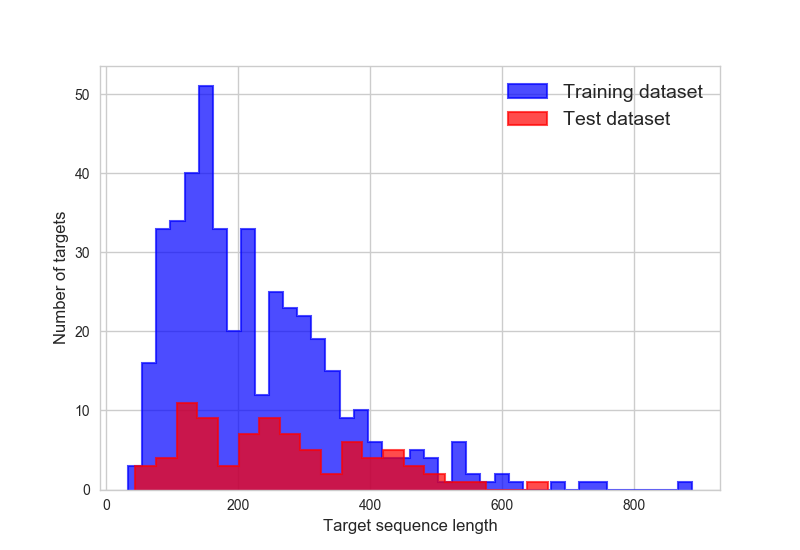
\includegraphics[width=\linewidth]{Fig/datasetLengthDistributions.png}
    \caption{The distributions of sequence lengths for targets in training set(blue) and test set(red).}
    \label{Fig:dataLengthDist}
\end{figure}

\begin{table}[H]
\begin{center}
\begin{tabular}{ c | c | l }
    
    Test set ID & Closest training set ID & E-value \\
    \hline
    T0768 & T0690 & 2.70e-13\\
    T0770 & T0645 & 1.79e-13\\
    T0772 & T0518 & 1.89e-07\\
    T0776 & T0707 & 3.98e-05\\
    T0783 & T0699 & 1.19e-22\\
    T0798 & T0308 & 9.57e-06\\
    T0813 & T0398 & 2.45e-05\\
    T0819 & T0636 & 8.66e-15\\
    T0854 & T0324 & 2.13e-13\\
\end{tabular}
    
    \caption {The closest homologs from training and test sets. The search was performed using blastp tool. The database was constructed from 
    the training set sequences; test sequences were queried against this database. We used 1e-4 e-value cutoff to filter only significant 
    alignments.}
    \label{Tbl:datasetsSimilarity}
\end{center}
\end{table}


\begin{table}[H]
\begin{center}
\begin{tabular}{ l | l | l }

    Common family & Test set target & Train set targets \\
    \hline
    PF00795.21 & T0794 & T0542 \\ \hline
    PF13472.5 & T0776 & T0448, T0297, T0286, T0750 \\ \hline
    PF03807.16 & T0813 & T0398, T0393, T0702 \\ \hline
    PF00266.18 & T0801 & T0339, T0697 \\ \hline
    PF01128.18 & T0783 & T0699, T0420 \\ \hline
    PF07949.11 & T0780 & T0572 \\ \hline
    PF13577.5 & T0815 & T0752, T0736 \\ \hline
    PF12804.6 & T0783 & T0593, T0699, T0420 \\ \hline
    PF13242.5 & T0854 & T0371, T0341, T0303, T0324, T0330, T0329, T0418 \\ \hline
    PF13306.5 & T0768 & T0690, T0671, T0713, T0653 \\ \hline
    PF12741.6 & T0770 & T0664, T0645, T0532 \\ \hline
    PF00025.20 & T0798 & T0308 \\ \hline
    PF12872.6 & T0792 & T0549 \\ \hline
    PF03446.14 & T0813, T0851 & T0398, T0393, T0702 \\ \hline
    PF00155.20 & T0801, T0819 & T0591, T0636, T0436, T0697 \\ \hline
    PF13419.5 & T0854 & T0371, T0341, T0303, T0379, T0324, T0330, T0329, T0418, T0635 \\ \hline
    PF12680.6 & T0815 & T0451, T0475 \\ \hline
    PF06439.10 & T0772 & T0518 \\ \hline
    PF12771.6 & T0770 & T0664, T0645, T0532 \\ \hline
    PF08477.12 & T0798 & T0308 \\ \hline
    PF00657.21 & T0776 & T0297, T0286, T0679 \\ \hline
    PF00071.21 & T0798 & T0308 \\ \hline
    PF00702.25 & T0854 & T0303, T0324, T0330, T0329, T0418, T0635 \\ \hline
    PF01926.22 & T0798 & T0308 \\ \hline
    PF12697.6 & T0764 & T0672 \\ \hline
\end{tabular}
    
\caption {Targets from test and train sets that belong to the same PFam family \cite{}. To obtain the family of a target we used HMMER search \cite{}.
Out of 564 targets in training and 83 targets in test sets 403 and 65 targets correspondingly had the families assigned to them. In total, this 
table contains 25 families, that correspond to the distinct 25 PFam clans. Alltogether, this table contains 16 test targets and 42 training targets.}
\label{Tbl:SharedPFam}
\end{center}
\end{table}

\begin{figure}[H]
    \centering
    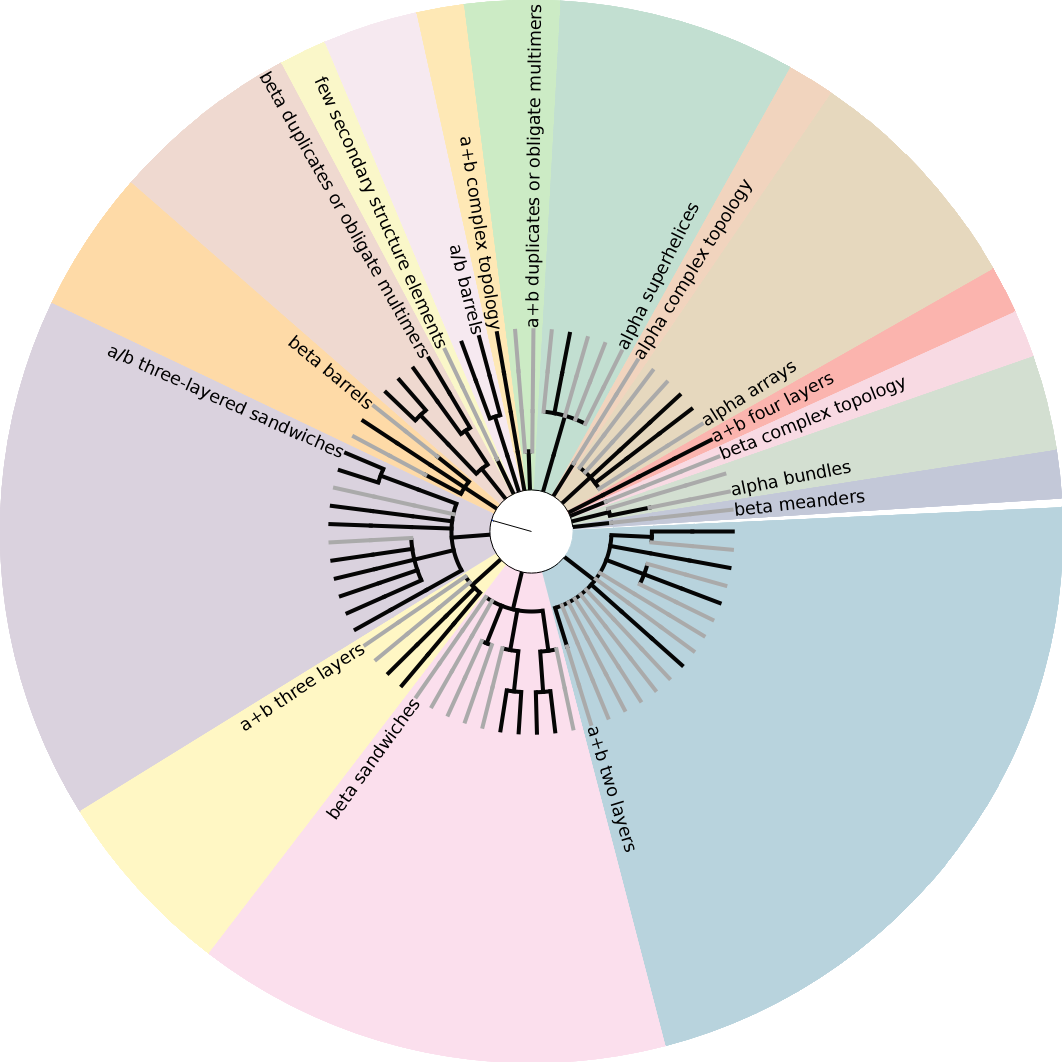
\includegraphics[width=\linewidth]{Fig/folds_graph.png}
%
    \caption{Classification of the test set structures into the lower
    four ECOD structural levels (from the center out): architecture
    (A), possible homology (X), homology (H), and topology (T). The
    names of the architecture types are shown in the outer circle of
    the diagram.
%%% Why do you have two different architecture names in the same A
%%% group? (brown color: ``alpha complex topology'' and ``alpha
%%% arrays'')
    The grey lines denote test set classes that have no
    respective representative in the training set. The black lines
    show the classes that have representatives in both training and
    test sets. We do not show the F-groups because they have litle
    overlap among the training and test sets.
%%% Why not showing the F-groups?
}
%
    \label{Fig:foldsGraph}
\end{figure}

\begin{figure}[H]
    \makebox[\textwidth]{
    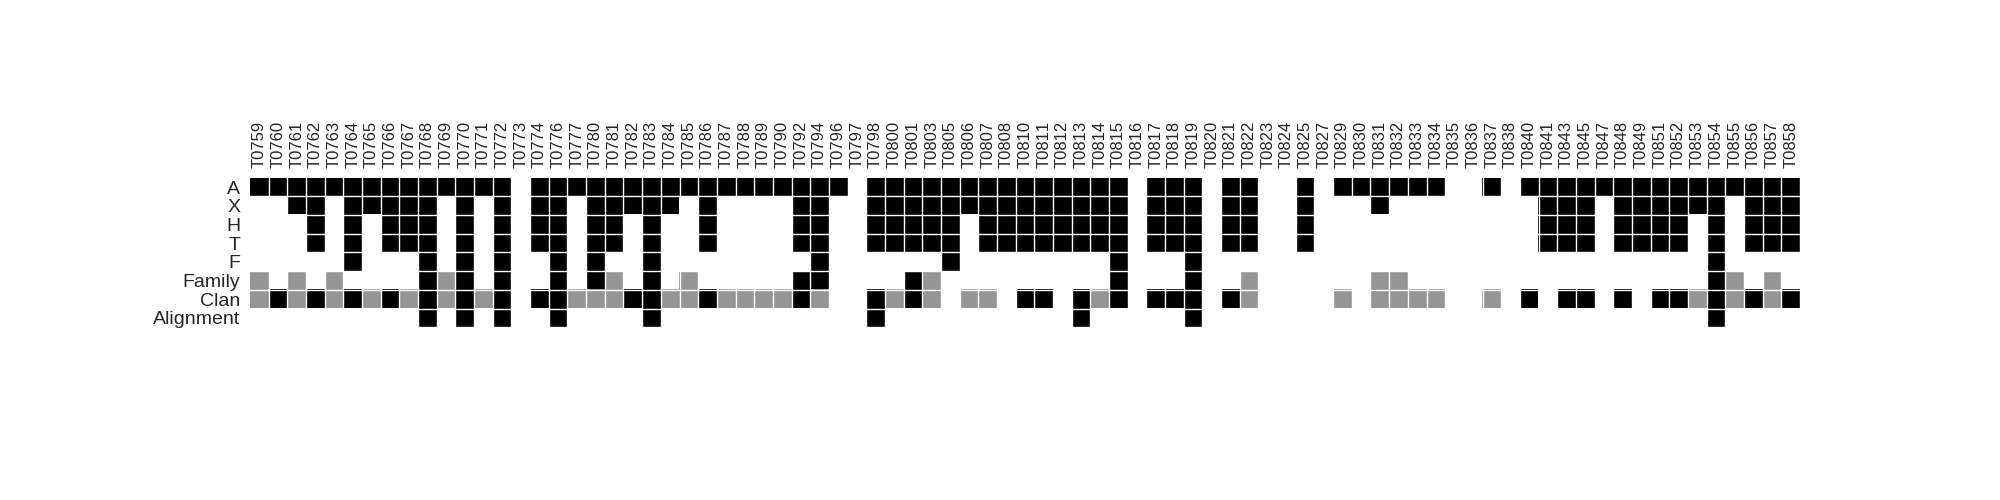
\includegraphics[width=\paperwidth]{Fig/summary_table.png}
    }
%
    \caption{Overlap of the training set on each target domain of the
    test set (from T0759 to T0858). The first 5 rows of tiles
    correspond to the ECOD classification of protein domains (A-, X-,
    H-, T-, and F-groups). A black tile in any of these rows indicates
    that at least one structure from the training set belongs to the
    same ECOD group as the target. Targets for which no ECOD
    classification is available are left empty.
%%% I see that all targets excluded from the analysis have an empty
%%% row of squares. Is T0838 excluded as well? What about the targets
%%% that are not in the list? (775, 778, 779, 791, 793, 795, etc.)
%%% Were they excluded from the CASP competition?
    A black tile in the ``Family'' row indicates that at least one
    structure from the training set belongs to the same Pfam family as
    the target. (A grey tile indicates that no Pfam family information
    is available for the target.) The ``Clan'' row shows similar
    information for Pfam clans. A black tile in the ``Alignment'' row
    indicates that at least one sequence in the training set aligns to
    the target sequence with an E-value smaller than $10^{-4}$.}
%
    \label{Fig:summaryTable}
\end{figure}
